\chapter{Quantum network of neutral atom clocks}
\label{ch:Komar2015}
%%%%%%%%%%%%%%%%%%%%%%%%%%%%%%%%%%%%%%%%%%%%%%%%

%%%%%%%%%%%%%%%%%%%%%%%%%%%%%%%%%%%%%%%%%%%%%%%%%%%%%%%%%%%%%%%%%%%%%%%%%%%%%%%%%%5
%%%%%%%%%%%%%%%%%%%%%%%%%%%%%%%%%%%%%%%%%%%%%%%%%%%%%%%%%%%%%%%%%%%%%%%%%%%%%%%%%%5
\section{Introduction} 
%%%%%%%%%%%%%%%%%%%%%%%%%%%%%%%%%%%%%%%%%%%%%%%%%%%%%%%%%%%%%%%%%%%%%%%%%%%%%%%%%%5
%%%%%%%%%%%%%%%%%%%%%%%%%%%%%%%%%%%%%%%%%%%%%%%%%%%%%%%%%%%%%%%%%%%%%%%%%%%%%%%%%%5
The current record in clock precision is held by ytterbium and strontium clocks
\cite{Ludlow2015}, capable of reaching $\sim 10^{-18}$ total fractional
frequency uncertainty. Apart from the enormous amount of effort and innovation,
this unprecedented accuracy was attainable due to the large number of clock
atoms ($10^3-10^4$) \cite{Hinkley2013, Bloom2013, Nicholson2015}.
In our recent work \cite{Komar2014}, we showed that a quantum network of atomic
clocks can result in substantial boost of the overall accuracy if multiple
clocks are connected in quantum entanglement. The proposed globally entangled
state, Greenberger-Horne-Zeilinger (GHZ) state, is more sensitive to the global
phase evolution of the clock atoms, and allows for an improved measurement of
the passage of time. If the GHZ state is set up and interrogated in the optimal
way \cite{Kessler2014, Berry2009}, frequency measurements can asymptotically
reach the Heisenberg limit \cite{Hall2012}, associated with the total number of
atoms in the entire network.
 
Imperfections during creation of the GHZ state are the main obstacles for
experimental realizations of a quantum clock network. Errors arising during the
distribution of entanglement add up, and limit the total number of atoms and
clocks with which the fidelity does not drop significantly. Efforts are being
made to make both the non-local \cite{sangouard3} and local entanglement
distribution \cite{Sorensen1999, Saffman2010} faster and more reliable. Of
particular interest are applications of these ideas to neutral atom clocks.

In this Letter, we show how a non-local  GHZ state can be created across
multiple, spatially separated neutral atom clocks with high fidelity. Our
protocol relies on strong Rydberg blockade for enhancing local atom-atom
interaction, collective excitations for enhancing photon-atom interaction, and
single photon quantum channels at telecom frequency for reliable non-local
connections. We propose and analyze a realization using neutral Yb ensembles,
suitable for the current atomic clock technology.

Rydberg blockade is a result of the interaction arising between atoms excited to
Rydberg states in an ensemble. If driven resonantly, the first excited atom
blocks the transition of a second one, thus at most one atom can get coherently
excited to the Rydberg state \cite{Dudin2012, Dudin2010, Ebert2015}, allowing
precise quantum control. Rydberg blockade has been proposed as an efficient tool
to realize quantum gates and perform quantum information processing
\cite{Lukin2001, Muller2009, Saffman2010, Zhao2010, Han2010, Goerz2014}.
Different ways of trapping and manipulating Rydberg states are currently  under
investigation both  experimentally \cite{Chen2010, Bariani2012,
Firstenberg2013, Antezza2014, Weber2015} and theoretically \cite{Topcu2013,
Beterov2013, Topcu2014}.



%%%%%%%%%%%%%%%%%%%%%%%%%%%%%%%%%%%%%%%%%%%%%%%%%%%%%%%%%%%%%%%%%%%%%%%%%%%%%%%%%%5
%%%%%%%%%%%%%%%%%%%%%%%%%%%%%%%%%%%%%%%%%%%%%%%%%%%%%%%%%%%%%%%%%%%%%%%%%%%%%%%%%%5
\section{Description of the protocol}
%%%%%%%%%%%%%%%%%%%%%%%%%%%%%%%%%%%%%%%%%%%%%%%%%%%%%%%%%%%%%%%%%%%%%%%%%%%%%%%%%%5
%%%%%%%%%%%%%%%%%%%%%%%%%%%%%%%%%%%%%%%%%%%%%%%%%%%%%%%%%%%%%%%%%%%%%%%%%%%%%%%%%%5

We describe our protocol for $K$ identical atomic clocks arranged in a sequence,
each connected to its neighbors with optical channels, and each using $n$
identical atoms, trapped in an optical lattice.
We use the atomic levels, shown on \reffig{fig:steps123}(a) for our protocol:
The two levels of the clock transition, $g, f$, a metastable shelving level $s$, an
excited level $e$, which spontaneously decays to $g$, and two strongly
interacting Rydberg levels, $r_1$ and $r_2$.
We further require transitions between levels, marked with arrows, to be driven
independently.

We imagine preparing all atoms in the ground state $g$, after which
our protocol consists of five subsequent steps.
First, using blockade, we create two independent collective excitations in
each ensemble, using two separate atomic levels ($f$ and $s$).
Second, each ensemble emits single photon pulses that are entangled with one of these
collective excitations.
Third, the photons are sent towards the neighboring atomic clocks, and measured
with a linear optics setup in Bell-basis. Fourth, upon success, each clock
performs a local CNOT operation to connect the two collective excitations. The
result is a set of $K$ entangled collective excitations, one in each clock,
which serve as "seeds" for a global GHZ state.
In the fifth, and final, step the clocks locally "grow" a GHZ state out of each
seed, and thus a global GHZ state is obtained. In the following, we provide detailed description and analysis of these five steps, discuss the specific realization in Yb atoms and analyze most important sources of imperfections and errors. 



%%%%%%%%%%%%%%%%%%%%%%%%%%%%%%%%%%%%%%%%%%%%%%%%%%%%%%%%%%%%%%%%%%%%%%%%%%%%%%%%%%5
\subsection{Collective excitations}
%%%%%%%%%%%%%%%%%%%%%%%%%%%%%%%%%%%%%%%%%%%%%%%%%%%%%%%%%%%%%%%%%%%%%%%%%%%%%%%%%%5
In the first step, we make use of the Rydberg blockade to create a superposition
of one and zero excitation in both $f$ and $s$ levels, following the approach of \cite{Lukin2001, Saffman2010,Dudin2012}.
This is done by performing the following sequence of driving pulses:
$[\pi/(2\sqrt{n})]_{g,r1}$, $[\pi]_{f,r1}$, $[\pi]_{f,s}$,
$[(\pi/(2\sqrt{n})]_{g,r1}$, $[\pi]_{f,r1}$, shown
on \reffig{fig:steps123}(a), where $[\phi]_{a,b}$ stands for a
pulse with total, single-atom Rabi phase $\phi$ between level $a$ and $b$.
Starting from the state $\ket{g}^{\otimes n} =: \ket{0}$, this pulse sequence creates the state
\bel
\label{eq:step1}
(1 + f\+) (1 + s\+) \ket{0} =:
\Big(\ket{0_f} + \ket{1_f}\Big) \Big(\ket{0_s} + \ket{1_s}\Big), 
\eel 
where $f\+$
and $s\+$ are creation operators of the two (approximately) independent spin
wave modes, supported by the two levels $f$ and $s$. 

\begin{figure}
\centering
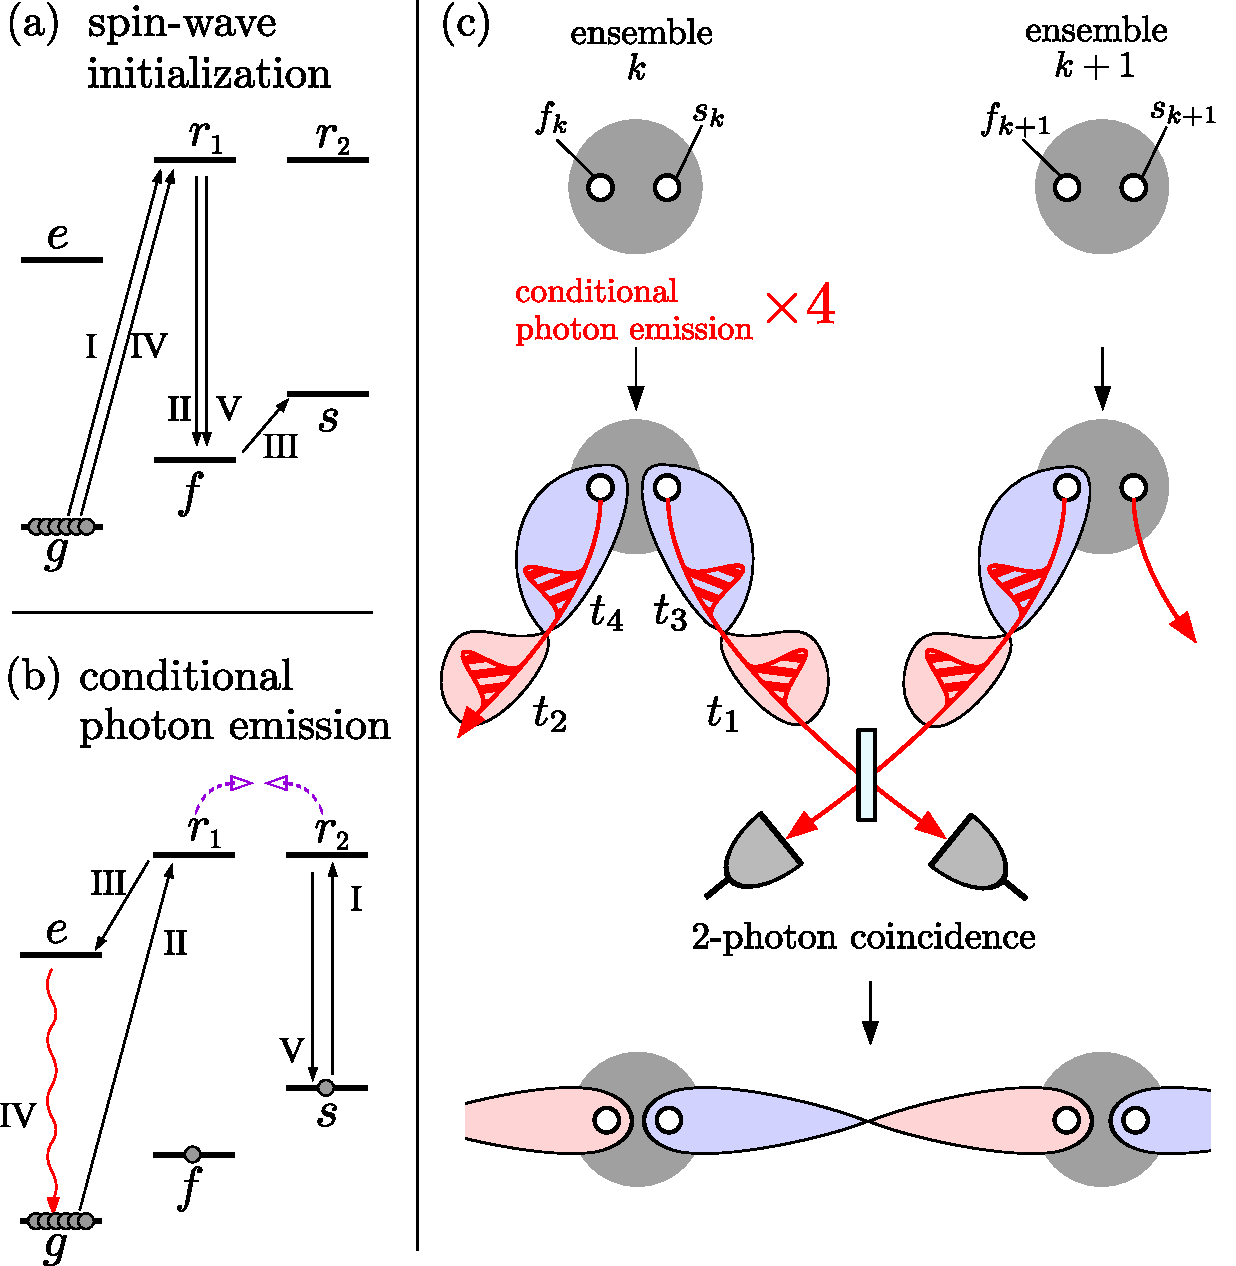
\includegraphics[width=0.8\textwidth]{./figs_Komar2015/steps123_1.pdf}
\caption
[Steps to generate of pairwise entanglement]
{
\label{fig:steps123}
Steps to generate pairwise entanglement. (a) Pulse
sequence used to initialize the spin-waves $f$ and $s$ in an ensemble.
(b) Pulse sequence inducing a conditional photon emission, the emitted photon
becomes entangled with the spin state $s$. 
(c) In three steps, neighboring ensembles generate pairwise entanglement between
their collective excitations. First, they induce $0+1$ superpositions of the two
independent spin waves, $f\+$ and $s\+$. Then applying the conditional photon
emission sequence four times, they emit four pulses, containing two
photons total. Each pair of photons is correlated with a unique spin state.
Finally, photons are measured with a linear optics setup, and 2-photon coincidences
indicate the creation of entanglement between neighboring ensembles.}
\end{figure}


%%%%%%%%%%%%%%%%%%%%%%%%%%%%%%%%%%%%%%%%%%%%%%%%%%%%%%%%%%%%%%%%%%%%%%%%%%%%%%%%%%5
\subsection{Non-local connection}
%%%%%%%%%%%%%%%%%%%%%%%%%%%%%%%%%%%%%%%%%%%%%%%%%%%%%%%%%%%%%%%%%%%%%%%%%%%%%%%%%%5
In the second step, spin-photon entangled states, using the spin wave modes $f$
and $s$, are created, using the an extended version of the scheme described in
\cite{Li2013}. Each spin-photon entangled state is created by the pulse sequence
shown on \reffig{fig:steps123}(b), involving $[\pi]_{s,r2}$,
$[\pi/\sqrt{n}]_{g,r1}$, $[\pi]_{e,r1}$, $[\pi]_{s,r2}$. With additional pulses
applied before and after this sequence flipping the states of $f$ and $s$ waves,
and proper timing, this is repeated four times to produce four time-bin
separated light pulses, which are entangled with the two spin waves,
\bal
	&& \Big(
	\ket{0_f}\ket{t_2} + \ket{1_f}\ket{t_4}
	\Big)
	\Big(
	\ket{0_s}\ket{t_1} + \ket{1_s}\ket{t_3}
	\Big)
\label{eq:step2}
\eal
where $\ket{t_j}\ket{t_k}$ is a two photon state with photons emitted at times
$t_j$ and $t_k$.


%%%%%%%%%%%%%%%%%%%%%%%%%%%%%%%%%%%%%%%%%%%%%%%%%%%%%%%%%%%%%%%%%%%%%%%%%%%%%%%%%%5
% Photon detection
%%%%%%%%%%%%%%%%%%%%%%%%%%%%%%%%%%%%%%%%%%%%%%%%%%%%%%%%%%%%%%%%%%%%%%%%%%%%%%%%%%5
In the third step, pairs of time-bin encoded photon pulses from two neighboring
ensembles are detected by interfering the two pulses on a beam splitter and
measuring two-photon coincidences \cite{duan3, Honjo2007, Rubenok2013}.
As a result, entangled states between neighboring atomic ensembles, $k$ and
$k+1$, are created \cite{Lukin2003, Shwa2013},
\bel
	\ket{0_s}_k\ket{1_f}_{k+1} \pm \ket{1_s}_k \ket{0_f}_{k+1},
\eel
where the individual kets represent the states of $f$ and $s$ spin waves in the
two ensembles, see \reffig{fig:steps123}(c).



%%%%%%%%%%%%%%%%%%%%%%%%%%%%%%%%%%%%%%%%%%%%%%%%%%%%%%%%%%%%%%%%%%%%%%%%%%%%%%%%%%5
\subsection{Local connection}
%%%%%%%%%%%%%%%%%%%%%%%%%%%%%%%%%%%%%%%%%%%%%%%%%%%%%%%%%%%%%%%%%%%%%%%%%%%%%%%%%%5
In the fourth step, the ensembles perform a local CNOT operation on the two
collective degrees of freedom, $f\+$ and $s\+$. This is done with the
following pulse sequence, $[\pi]_{s,r2}$, $[\pi]_{f,r1}$,
$[\pi/\sqrt{n}]_{g,r1}$, $[\pi]_{f,r1}$, $[\pi]_{s,r2}$, shown on
\reffig{fig:connection}(a), which promotes any population in $s$ to $r_2$, which
then blocks the path through $r_1$. The result is a
conditional flip $\ket{0_f} \leftrightarrow \ket{1_f}$, conditioned on having zero $s\+$ excitations. If we perform
$f\leftrightarrow s$ swaps before and after this process, we get a coherent flip
between $\ket{0_f, 0_s} \leftrightarrow \ket{0_f, 1_s}$. 

To understand the resulting state, let us consider two
entangled links, connecting three neighboring ensembles $k-1,k$ and
$k+1$ as shown on \reffig{fig:connection}(b). The corresponding state, before
the fourth step, is
\bel 
	\big(\ket{0,1} + \ket{1,0}\big)_{s_{k-1},f_k}
	\otimes
	\big( \ket{0,1}  + \ket{1,0}  \big)_{s_k,f_{k+1}},
\eel
where $\ket{n_{s_{k-1}}, n_{f_k}}\otimes\ket{n_{s_k},n_{f_{k+1}}}$ indicate the
number of excitations in the modes $s_{k-1}, f_k, s_k, f_{k+1}$ of the three
ensembles.
After the conditional flip of $s_k$ and measurement of $n_{s_k} \rightarrow m
\in \{0,1\}$, the state becomes $\ket{0,1, 1-m} + \ket{1,0,m}$, where the
remaining kets stand for $\ket{n_{s_{k-1}}, n_{f_k}, n_{f_{k+1}}}$.
Depending on the outcome, either only $f_k$ (if $n_{s_k} \rightarrow 1$) or the
entire right hand side (if $n_{s_k} \rightarrow 0$) needs to be flipped in order
to obtain the desired GHZ state, $\bigotimes_k \ket{0_f}_k + \bigotimes_k
\ket{1_f}_k$, of the $f$ excitations of each ensemble, $k = 1,2,\dots K$.
\begin{figure}
\centering
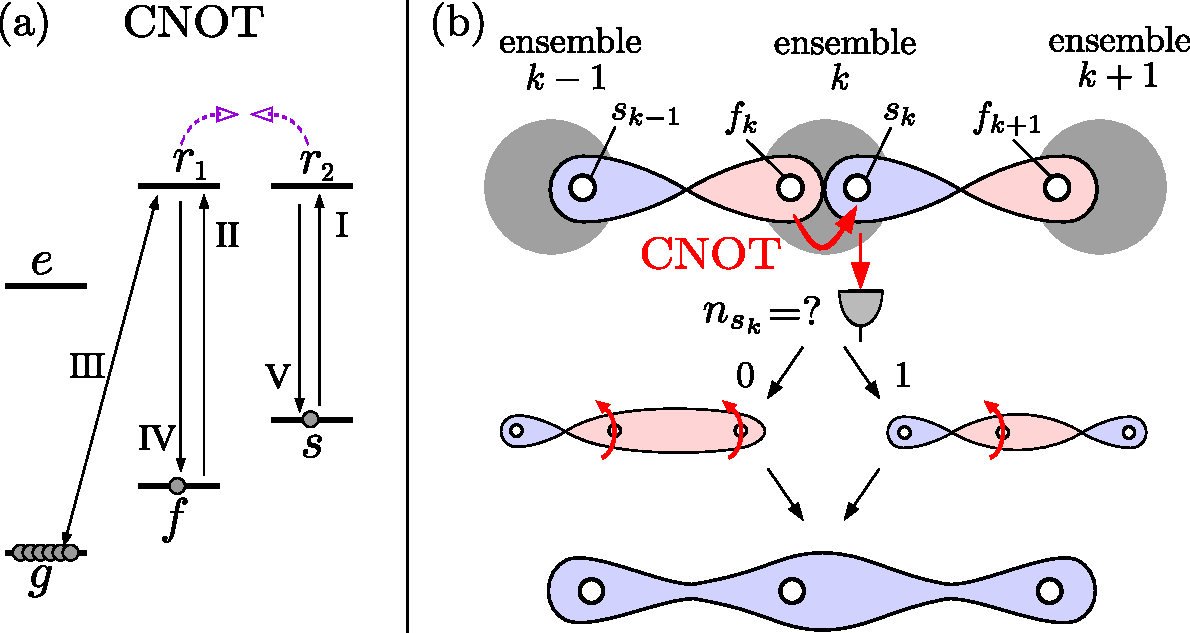
\includegraphics[width=0.8\textwidth]{./figs_Komar2015/connection_6.pdf}
\caption
[Connecting links into non-local GHZ state]
{
\label{fig:connection} 
Connecting links into non-local GHZ state.
(a) CNOT gate between
the two excitations $f$ and $s$: If level $s$ is occupied, then the coherent
(de)excitation of the $f$ level is blocked by the Rydberg blockade between
the $r_1$ and $r_2$ intermediate levels, otherwise it succeeds. 
(b) Connecting two entanglement links. The local CNOT and measurement
operations on ensemble $k$ entangle the two, initially independent, parts of
the system:
$s_{k-1}, f_k$ and $s_k, f_{k+1}$. Depending on the
outcome of the measurement, either only $f_k$, or the entire
right hand side needs to be flipped, in order to arrive to the proper GHZ
state.}
\end{figure} 


%%%%%%%%%%%%%%%%%%%%%%%%%%%%%%%%%%%%%%%%%%%%%%%%%%%%%%%%%%%%%%%%%%%%%%%%%%%%%%%%%%5
\subsection{Local GHZ growing}
%%%%%%%%%%%%%%%%%%%%%%%%%%%%%%%%%%%%%%%%%%%%%%%%%%%%%%%%%%%%%%%%%%%%%%%%%%%%%%%%%%5
In the fifth step, each ensemble locally expands the entanglement from its $f$
degree of freedom to all atoms using a collective Rydberg gate introduced in
Refs.
\cite{Saffman2009, Weimer2010}.
Since the previous steps have already entangled the $f$ excitations across the
ensembles, a transition that conditionally excites all local atoms will create a
global GHZ state of every atom in the network. The pulse sequence $[\pi]_{f,s}$,
$[\pi]_{s,r2}$, $[\pi/2]_{g,f}$, $[\pi(\Delta)]_{g,r1}$, $[\pi/2]_{g,f}$,
$[\pi]_{s,r2}$, shown in \reffig{fig:GHZ}(a),  does exactly that, where
$[\pi(\Delta)]_{g,r1}$ is an off-resonant dressing pulse, whose Rabi frequency
$\Omega$ and duration is set properly in order to introduce a conditional $\pi$
phase shift on level $g$.
This sequence transfers the atoms from $g$ to $f$ only if $r_2$ is unoccupied,
and gets blocked otherwise. The result is
\bel
\label{eq:step5}
	\bigotimes_{k=1}^K\ket{0_f}_k  + \bigotimes_{k=1}^K\ket{1_f}_k
	\;\rightarrow\; \bigotimes_{k=1}^K \ket{f}^{\otimes n} + \bigotimes_{k=1}^K
	s\+\ket{g}^{\otimes n},
\eel
where $\ket{f}$ and $\ket{g}$ denote the state of a single atom.
Finally, we get rid of
the $s$ excitation with a series of pulses that move it back to $g$:
$[\pi]_{f,s}$, $[\pi]_{f,r1}$, $[\pi]_{f,s}$, $[\pi/\sqrt{n}]_{g,r1}$, and end
up with $\ket{f}^{\otimes Kn} + \ket{g}^{\otimes Kn}$, a fully entangled state
of all $N = Kn$ atoms in the network. 
\begin{figure}
\centering
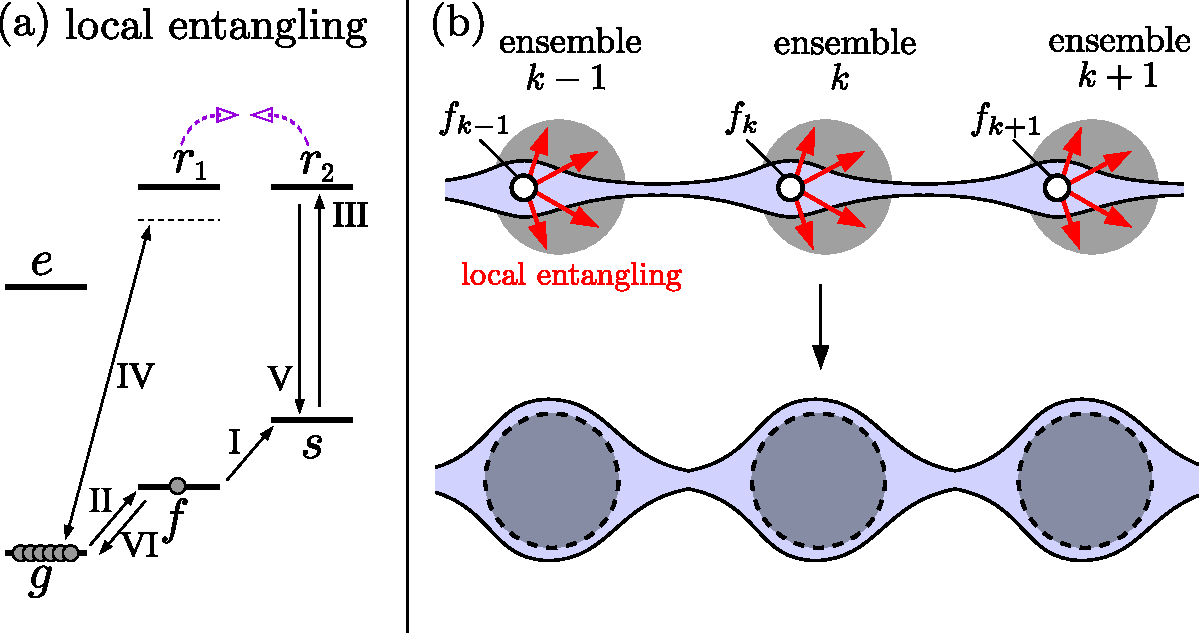
\includegraphics[width=0.8\textwidth]{./figs_Komar2015/GHZ_2.pdf}
\caption
[Local GHZ creation]
{  
\label{fig:GHZ}
Local GHZ creation.
(a) Conditional,
local GHZ state generation: Any excitation in level $s$ prevents the dressing of
$g$ with $r_1$, which, otherwise introduces a $\pi$ phase shift on $g$. With the
conjugation of $\pi/2$ pulses II and VI, this results in a transfer
from $g$ to $f$ conditioned on the population of $s$. (b) The local entangling
operation extends the GHZ state from the $f$ spin-wave to all atoms. As a result, every atom in the network gets entangled. }
\end{figure}

%%%%%%%%%%%%%%%%%%%%%%%%%%%%%%%%%%%%%%%%%%%%%%%%%%%%%%%%%%%%%%%%%%%%%%%%%%%%%%%%%%5
%%%%%%%%%%%%%%%%%%%%%%%%%%%%%%%%%%%%%%%%%%%%%%%%%%%%%%%%%%%%%%%%%%%%%%%%%%%%%%%%%%5
\section{Implementation}
%%%%%%%%%%%%%%%%%%%%%%%%%%%%%%%%%%%%%%%%%%%%%%%%%%%%%%%%%%%%%%%%%%%%%%%%%%%%%%%%%%5
%%%%%%%%%%%%%%%%%%%%%%%%%%%%%%%%%%%%%%%%%%%%%%%%%%%%%%%%%%%%%%%%%%%%%%%%%%%%%%%%%%5
We next investigate  the robustness of our  protocol  in  light of realistic physical imperfections. 
We assume that all imperfections decrease the coherence between the two
components of the GHZ state, and therefore the fidelity can be written as
$F = [1 + \exp(-\eps_\mathrm{tot})]/2$, where $\eps_\mathrm{tot}$ is the sum of the
errors.
The errors arising during each non-local connection step
$\eps_\mathrm{non-local}$ and the errors arising during a local GHZ creation
in one clock $\eps_\mathrm{local}$ add up to the total error $\eps_\mathrm{tot} =
(K-1)\eps_\mathrm{non-local} + K\eps_\mathrm{local}$, and overall fidelity
\bel
	F \geq \left\{1+ \exp\left[-N\left(\frac{\eps_\mathrm{non-local}}{n}
	+ \frac{\eps_\mathrm{local}}{n}\right)\right]\right\} /2.
\eel
The error, $\eps_\mathrm{tot}$, increases linearly with the total
number of atoms in the network, $N$, and the coefficient,
$(\eps_\mathrm{non-local} + \eps_\mathrm{local})/n$, depends on the number of atoms,
$n$, at a single site. For a certain optimal local atom
number $n_\mathrm{opt}$, the total fidelity is maximal, i.e.
decreases with the slowest rate, as $N$ increases. Evenly distributing
the atoms into $K_\mathrm{opt} = N/n_\mathrm{opt}$ groups is therefore optimal.


To be specific, we focus on a possible implementation of our scheme with
ensembles of neutral ytterbium atoms whose relevant electronic levels are shown on
\reffig{fig:Yb_levels}.
\begin{figure}[h]
\centering
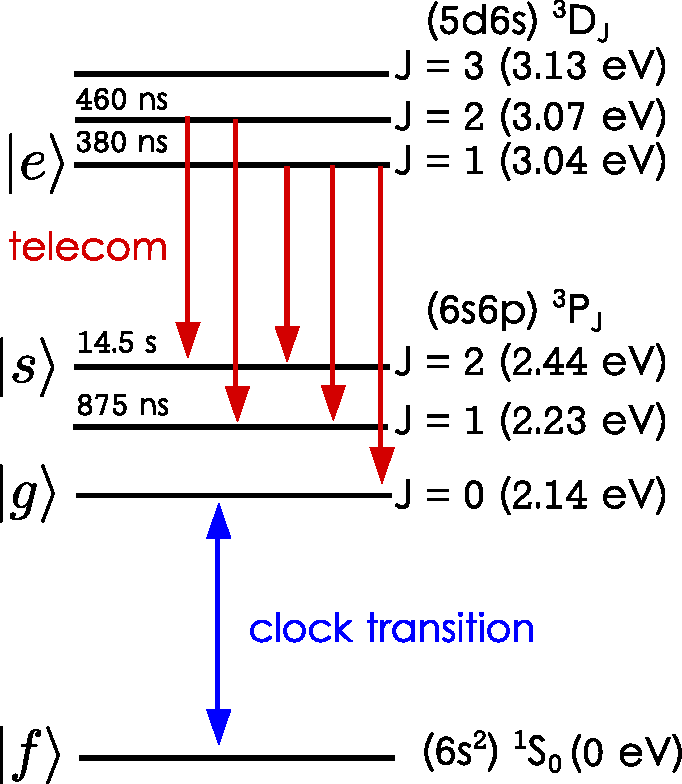
\includegraphics[width=0.45\textwidth]{./figs_Komar2015/Yb_levels.pdf}
\caption
[Implementation with Yb levels]
{ 
\label{fig:Yb_levels}
Implementation of our protocol in the lower level of neutral Yb. We assign
the roles of $g$ and $f$ to the clock levels, the role of $s$ to the metastable
$J=2$ level of $6s6p$, and the role of $e$ to the $J=1$ level of the excited
state $5d6s$, which spontaneously decays to all three levels of $6s6p$ state by
emitting a telecom frequency photon.}
\end{figure}
We identify the  following levels of neutral
Yb  relevant for our protocol:
$\ket{g} =
\ket{6s6p({}^3\!P_0)}$, $\ket{f} = \ket{6s^2({}^1\!S_0)}$, $\ket{s} =
\ket{6s6p({}^3\!P_2)}$ and $\ket{e} = \ket{5d6s({}^3\!D_1)}$, and two Rydberg
levels $\ket{r_1} = \ket{6s\tilde n s({}^1\!S_0)}$ and $\ket{r_2} =
\ket{6s\tilde n p_{m=+1}({}^1\!P_1)}$ with the same principle
quantum number $\tilde n$. 
Although the branching ratio for $e\rightarrow g$ decay is not unity, the
large population in $g$ collectively enhances this decay channel, and the
transition becomes effectively closed. Due to the different symmetries of these
states, the coherent coupling between $f,e, s$ levels and the Rydberg levels
$r_1, r_2$ need to be created via two-photon transitions. We imagine the atoms
being held in position by a 2D or 3D optical lattice with period $a =
275.75~\mathrm{nm}$, each potential minimum holding a single Yb atom. (The lattice
intensity can be modulated during the Rydberg state excitation
\cite{Tiecke}.)  (We found that the performance difference between the 2D
and 3D lattice is less than a factor of two. See Appendix \ref{app:clock_precision}.)
% The quantization axis is set perpendicular to the plane of
% the lattice, which ensures that the dipole-dipole interaction between
% $\ket{r_1}$ and $\ket{r_2}$ states depends only on spatial separation. 
 
We consider the following errors in our analysis. During
non-local connection, we take into account the finite $r_1$-$r_2$ interaction, which
allows the creation of an $r_1$ excitation with some small probability, even if
$r_2$ is populated, the finite lifetime of the $s$ and $r_2$ levels, the
non-zero branching ratio during the decay of $e$ into states other than $g$, and
the dark-count rate of photo-detectors. For the local GHZ creation step, we account
for the same imperfection of the
$r_1$-$r_2$ blockade as for the non-local entangling step, the finite lifetimes
of the Rydberg levels $r_1$ and $r_2$, and the inhomogeneous broadening of the
single excited Rydberg states due to their coupling to double-excited states,
induced by the driving field.
(See Appendix \ref{app:local_entanging_errors} and
\ref{app:non-local_entangling_errors} for details.) We estimate the effect of these errors, and numerically optimize the free parameters: the Rabi frequency
$\Omega$ and the detuning $\Delta$ of the dressing field, and the
number of local atoms $n$, for principle quantum numbers, $50\leq \tilde n \leq
150$ of the Rydberg levels, in order to find the minimal
error per atom, $E := \eps_\mathrm{tot}/N$.
 
To illustrate, for $\tilde n = 120$, we find the optimum at $n_\mathrm{opt} =
298$, $\Delta = 10.9\times 10^4 \,\gamma$ and $\Omega = 8.33\times
10^4\,\gamma$, where $\gamma \sim 1\,\mathrm{kHz}$ is the natural linewidth of the
Rydberg levels. In this case, the error per atom is $E_\mathrm{min}=
[\eps_\mathrm{tot}/N]_\mathrm{min} = 6.7\times 10^{-5}$ and the fidelity is
$F_\mathrm{max} = [1 + \exp(-6.7\times 10^{-5}\,N)]/2$.
% With this
% choice of parameters, we can also estimate the number of clocks $K_\mathrm{opt}$
% that can be optimally connected if a target fidelity of $F = 0.8$ is set. We
% find $K_\mathrm{opt} \leq -\log(2F - 1) / (E_\mathrm{min} n_\mathrm{opt}) = 5.2$. This
% means that we can entangle five clocks, each containing about 200
% atoms. 
Contributions of the different error sources are shown in Table
\ref{table:errors}. (See Appendix \ref{app:optimization} for more details.)
\begin{table}
\centering
\begin{tabular}{|l|c|c|}
\hline
 & error per atom & ratio in total\\
\hline
imperfect blockade & $1.41 \times 10^{-5}$ & 21\%\\
$r_1$ decay & $2.89 \times 10^{-5}$ & 43\%\\
$r_2$ decay & $6.62 \times 10^{-7}$ & 1\%\\
inhom. broadening & $6.62 \times 10^{-7}$ & 1\%\\
$r_2$ deacy (non-local) & $ \sim 10^{-10}$ & $<0.1$\%\\
photon detection & $ \sim 10^{-9}$ & $<0.1$\%\\
memory error & $ \sim 10^{-8}$ & $<0.1$\%\\
imperfect br. ratios & $2.26 \times 10^{-5}$ & 34\%\\
\hline
total error per atom & $6.70 \times 10^{-5}$ & 100\%\\
\hline
\end{tabular}
\caption
[Error budget]{
\label{table:errors}
The absolute and relative contribution of the different error sources to the
total error per atom $E$, at $\tilde n = 120$, $\Delta =
\Delta_\mathrm{opt} = 10.9\times 10^4\,\gamma$, $\Omega = \Omega_\mathrm{opt} = 
8.33\times 10^4\,\gamma$ and $n = n_\mathrm{opt} = 298$, for the 3D setup. (See
Appendix \ref{app:optimization} for 2D results.)}
\end{table}

%%%%%%%%%%%%%%%%%%%%%%%%%%%%%%%%%%%%%%%%%%%%%%%%%%%%%%%%%%%%%%%%%%%%%%%%%%%%%%%%%%5
%%%%%%%%%%%%%%%%%%%%%%%%%%%%%%%%%%%%%%%%%%%%%%%%%%%%%%%%%%%%%%%%%%%%%%%%%%%%%%%%%%5
\section{Clock network optimization}
%%%%%%%%%%%%%%%%%%%%%%%%%%%%%%%%%%%%%%%%%%%%%%%%%%%%%%%%%%%%%%%%%%%%%%%%%%%%%%%%%%5
%%%%%%%%%%%%%%%%%%%%%%%%%%%%%%%%%%%%%%%%%%%%%%%%%%%%%%%%%%%%%%%%%%%%%%%%%%%%%%%%%%5
With the optimal ensemble size $n_\mathrm{opt}$, determined above, we optimize the
remaining parameters of the clock network, namely the total number of entangled
atoms $N$ and the number of clocks $K$. Although having more atoms always
results in improved clock precision, entangling all available atoms is not
necessarily optimal. To see this, we compare the stability of the entangled
clock network and a non-entangled network, and find an optimal entangled atom
number $N_\mathrm{opt}$ by maximizing the precision gain over the non-entangled
scheme,
\bel
\label{eq:gainKomar2015}
	G = \frac{\sigma_\mathrm{non-ent}}{\sigma_\mathrm{ent}/(2F-1)} =
	e^{-EN}\frac{\pi}{8}\sqrt{\frac{N}{\log N}},
\eel 
where $\sigma_\mathrm{ent} = \frac{1}{\omega_0 \tau}\frac{8}{\pi}\frac{\sqrt{\log
N}}{N}$ (from \cite{Komar2014}, assuming perfect fidelity, and that $\tau$ is
smaller than the reduced atomic coherence time $\gamma_\mathrm{at}^{-1}/N$) and
$\sigma_\mathrm{non-ent} = \frac{1}{\omega_0\tau}\frac{1}{\sqrt{N}}$ (for $N$
independent atoms) are the Allan-deviations of the two schemes, where $\omega_0$
is the central frequency and $\tau$ is the total available measurement time.
The additional factor of $2F-1 = e^{-EN}$ is due to the reduced Fisher
information of a non-pure GHZ state, where $E$ is the error per atom and $F$
is the fidelity of the initial state.
(See supplementary materials for details.) For $E = E_\mathrm{min} = 6.7\times
10^{-5}$, \refeq{eq:gainKomar2015} is maximal at $N_\mathrm{opt} \approx
1/(2E_\mathrm{min}) \approx 7500$, where $G_\mathrm{max} = 6.9$, and $F =
[1+e^{-N_\mathrm{opt} E_\mathrm{min}}]/2 = 0.82$.

% Given that the optimal number of atoms at each clock is $n_\text{opt} \approx
% 300$, the optimal number of clocks is $K_\text{opt} = N_\text{opt} /
% n_\text{opt} \approx 22$. We can entangle 22 clocks, each consisting of $\sim
% 300$ atoms, and gain about  a factor of $\sim 7$ in terms of clock precision
% over the classical scheme. If multiples of 7500 atoms are available, then the
% best way to utilize them is to create multiple independent GHZ states (either in
% a single clock or in a network), and combine the measurement results
% classically. The overall gain of a factor of $7$ means that we can use $50$
% times less atoms to reach the same precision as any non-entangled clock
% (network).

The above optimum is achieved by 7500 atoms distributed in $K_\mathrm{opt} =
N_\mathrm{opt}/n_\mathrm{opt} \approx 22$ clocks. Since current lattice clocks can
employ $10^3-10^4$ atoms, we can imagine entangling this many atoms in
a single vacuum chamber. With realistic atom densities, the atoms need to be
separated into $\sim 10^2$ ensembles, for efficient Rydberg blockade. We imagine
using an individually addressed ``messenger'' atom, that can be moved to the
vicinity of each ensemble, and can be brought to entanglement with them using
dipole-dipole interaction.
(See Supplementary for more details.) Such a scheme is free from imperfections
affection the photons in the previous scheme, and thus can reach a higher
fidelity for a given number of atoms, or use more atoms to achieve a higher
gain. We find that, at the optimum, the gain over the classical scheme is $\sim
14$, twice the gain of the network scheme.


% Any additional clocks or atoms we are
% better off using to create copies of this construction, running them in
% parallel, and averaging the signals classically.



%%%%%%%%%%%%%%%%%%%%%%%%%%%%%%%%%%%%%%%%%%%%%%%%%%%%%%%%%%%%%%%%%%%%%%%%%%%%%%%%%%5
%%%%%%%%%%%%%%%%%%%%%%%%%%%%%%%%%%%%%%%%%%%%%%%%%%%%%%%%%%%%%%%%%%%%%%%%%%%%%%%%%%5
\section{Conclusion}
%%%%%%%%%%%%%%%%%%%%%%%%%%%%%%%%%%%%%%%%%%%%%%%%%%%%%%%%%%%%%%%%%%%%%%%%%%%%%%%%%%5
%%%%%%%%%%%%%%%%%%%%%%%%%%%%%%%%%%%%%%%%%%%%%%%%%%%%%%%%%%%%%%%%%%%%%%%%%%%%%%%%%%5

We presented and analyzed a protocol, capable of fully entangling ensembles of
neutral atoms located in different atomic clocks. Local interactions are made
robust by utilizing the strong interaction between Rydberg excitations, and
non-local entanglement creation is made reliable with strong atom-light
coupling, suppressed photon propagation errors and long atomic memory lifetimes.
We showed that our scheme, in particular a realization with neutral Yb
ensembles, is feasible and provides significant gain over non-entangled schemes
even in the light of physical imperfections. Our results provide the first
detailed proposal for a network that can serve as a first prototype of the
global quantum clock network outlined in \cite{Komar2014}.
